
\section{GPU Architecture}
Since the GPU backend of Accelerate only works with CUDA capable devices (see section \ref{sec:accelerate}), we will mostly focus on the architecture of newer NVidia GPUs.
Massive parallel workloads are executed on numerous cores clustered in streaming multiprocessors (SMs).
The memory is structured in a multi-level hierarchy containing an L1 cache for each SM, a shared L2 cache for all SMs and multiple banks of DRAM \cite{nvidia2017volta,nvidia2020ampere}.

When working with CUDA the programmer defines a kernel.
This is normally done with CUDA C++, an extension on C++ programming language, but in our case Accelerate will handle the generation of kernels (section \ref{sec:accelerate}) \cite{nvidia2021cudadocs}.

\subsection{Hardware}
On modern Nvidia GPU architectures the compute units are grouped in graphics processing clusters (GPC).
Since GPUs are primarily used in graphics applications, the GPC contains some specialized components: a raster engine, Texture Processing Clusters (TPCs), \TODO{\dots}.
The main point of interest are streaming multiprocessors (SMs) in the TPCs.
Each SMs has its own instruction scheduler and various execution pipelines.
\citeauthor{jia2019dissecting} suggests that a threadblock should contain at least 128 threads due to SMs on Turing, Volta, and Ampere being split into four processing blocks \cite{jia2019dissecting,nvidia2017volta,nvidia2018turing,nvidia2020ampere}.

\TODO{Link text with sketch}

\begin{figure}[!hb]
    \centering
    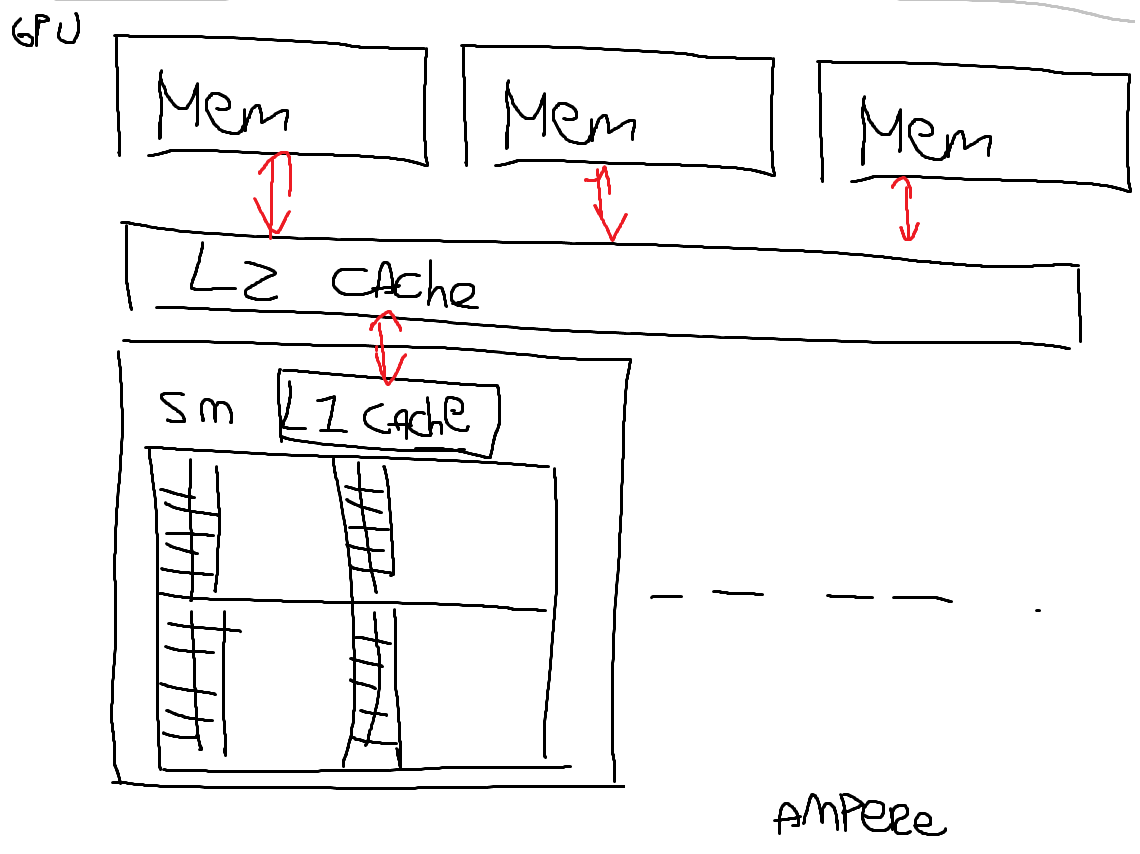
\includegraphics[width=8cm]{sketches/ampere_arch.png}
    \caption{
        Ampere sketch.
    }
\end{figure}

\TODO{Define + summerize architectures}
\TODO{More specific + figure}

\subsection{Software}
Executions on a GPU are directed on both the host and device (GPU).
\textit{Kernels} define the functions that should be executed on the GPU.
The host side controls how these kernels should be executed, namely how the threads should be launched and executed.
Threads are grouped and defined on a 2 level hierarchy: threads are grouped together in \textit{cooperative thread arrays} (CTAs), also known as thread blocks, and multiple CTAs can be queued for the execution of a single kernel.
Both can be controlled upon executing a kernel: the amount of threads per CTA (threadblock size) and the total amount of CTAs (gridsize).
CTAs get assigned to SMs in a round-robin fashion.

When an SM executes a CTA, it splits the work into warps, a grouping of 32-threads.
On architecture before Volta, a single warp is executed in a single instruction, multiple threads fashion, where a single program counter is shared amongst the 32 threads.
With the volta architecture, independent thread scheduling allows full concurency between threads and the scheduler can group multiple threads into SIMT units.

\TODO{SM can context switch between multipel warps to hide latency}

\TODO{Figure visualizing the whole thing because text is confusing... probably}

% random sketch
\begin{figure}[!hb]
    \centering
    \begin{tikzpicture}
        \pic at (0, 0) {thread};
        \pic at (2, 0) {threadblock};
        \pic at (5, 0) {warp};
    \end{tikzpicture}
    \caption{
        \TODO{remove this, only used to debug tikz pic codes}
    }
\end{figure}


\begin{figure}[!hb]
    \centering
    \begin{tikzpicture}
        \node at (1, 1.5) {threadblock size};
        \draw[decorate, thick, decoration={brace}] (0,1.1) --  (2,1.1);
        

        \node [rotate=90] at (-0.5, -1) {grid size};
        \draw[decorate, thick, decoration={brace}] (-0.1,-3.2) --  (-0.1,1);

        \pic at (0, 0) {threadblock};
        \pic at (0, -1.1) {threadblock};
        \pic at (0, -3.2) {threadblock};
    \end{tikzpicture}
    \caption{
        \TODO{host side workload assignment}
    }
\end{figure}

\subsection{GPU Caches}
\label{sec:cache_gpu}
To the programmer, the memory hierarchy is very simplified: there is the compute unit and the memory.
Caches are hidden from this model as on most architectures they are managed by hardware.

Memory can become a significant bottleneck due to the large amount of threads running concurrently.
Caches can alleviate this but are limited in size, and given a large enough problem can cause cache trashing -- the premature eviction of data before any significant reuse \cite{dai2016model}.
To improve efficiency of caches, caches asume spatial locality via cache lines.
A cache line is the smallest unit of data that a cache can hold.
For example, an L1 cache on a Turing GPU uses cache lines that hold 128 bytes of data.
Therefore, fetching data from memory also brings extra nearby data with it.

Data shared between threads through the cache can happen in a read-after-write (RAW) or read-after-read (RAR) manner.
RAW has data dependency between tasks, for example in scan operations.
RAR has no data dependency and can be executed in any order \cite{tripathy2021paver}.

The L1 cache in older Nvidia GPU architectures (Maxwell, Pascal) uses the least recently used (LRU) eviction policy.
When caches become full, we need to remove data (a cache line) from the cache to allow newer data to be cached.
An LRU eviction policy evicts data that is the least recently used.
\citet{jia2019dissecting} have shown that in Turing and Volta GPUs, the P-chase benchmark that is used to detect the LRU eviction policy presented by \citet{mei2016dissecting} fails to complete over the full L1 cache.
\citeauthor{jia2019dissecting} conclude that newer architectures (Turing, Volta) uses a non-LRU eviction policy \cite{jia2019dissecting, jia2018dissecting,mei2016dissecting}.
When the L1 cache in Turing and Volta GPU saturates, 4 consecutive cache lines are chosen randomly to be evicted.
This is in line with a new eviction policy mechanism introduced with Volta, where cache lines can be assigned a priority \cite{jia2019dissecting,nvidia2021cudadocs}.

Modern Nvidia GPUs are able to handle various types cache operations and eviction hints.
By default, loads are cached at all levels (L2, L1) with an LRU policy.
This brings a problem with it: if data is writen to a cached value, we need to evict this cache line from all other L1 caches first, since that value is no longer up to date after our update.
As an example, it is also possible to only cache on L2, bypassing L1.
Another option is to hint cache streaming, where the loaded cache line will have an evict-first policy to prevent polution of the cache.
Similar operations exist for writing data to memory.
In both cases it is up to the compiler and programmer to exploit this for extra performance \cite{nvidia2021cudadocs}.

\subsection{Performance of Access Patterns}
\citeauthor{lam1991cache} and \citeauthor{meyer2003algorithms} describe two types of reference reuse\cite{lam1991cache, meyer2003algorithms}:
\begin{itemize}
    \item \textbf{Spatial reuse} occurs when accessing data from the same cache line, increasing spatial locality.
    \item \textbf{Temporal reuse} occurs when the same data is accessed at a later time, increasing temporal locality.
\end{itemize}
The reuse factor can be kept track of by counting the two types of reuse.
Loading data horizontally (sequentially) exploits spatial locality and is therefore cheaper than loading data vertically.
Additionally, temporal reuse can only happen when other memory accesses do not displace reusable data from the cache.

\citeauthor{lam1991cache} proposed a method to model cache interference.
In the simplest case where all data used is cached in different locations (and therefore no data is evicted), the number of misses per variable $v$ is described by $D(v)/R(v)$, where $D(v)$ is the total number of references (loads) of $v$ and $R(v)$ is the reuse factor.
However, with interference misses when data gets displaced from cache, the total number of misses for $v$ is
\[
    D(v)\left(\frac{1}{R(v)}+\frac{R(v)-1}{R(v)}M(v)\right)
\]

With missrate being
\[
    M(v) = 1 \left(1 - S(v)\right) \prod_{u\in V - \{v\}}\left(1 - F(u)\right)
\]
$F(u)$ is defined as the fraction of cache used by variable $u$, and self interference $S(v)$ is defined to be the fraction of accesses that map to non-unique location in the cache.

\TODO{Illustrations for interference}


\section{CPU vs GPU based multi-threading}
\TODO{Aka, the limits of GPUs, segway to introduce Accelerate}

\section{Accelerate}
\TODO{Generalize to Array DSLs}
\label{sec:accelerate}
Accelerate is an embedded purely functional array language in Haskell \cite{chakravarty2011accelerating}.
Accelerate has a frontend containing the embedded language, and the backend which handles code generation and execution.
The frontend handles general optimizations such as sharing recovery and array fusion \cite{mcdonell2013optimising,balen2020optimal}.
Further hardware specific optimization is handled on the various backends.
There are two LLVM \cite{llvm} backends provided: one that targets multicore CPUs \texttt{accelerate-llvm-native} and one that targets Nvidia GPUs \texttt{accelerate-llvm-ptx}.
In both backends we compile Accelerate code to LLVM IR.
When we want to run Accelerate on a GPU, LLVM will handle the compilation from LLVM IR to PTX, the instructions set for Nvidia's CUDA programming environment \cite{mcdonell2015type, llvm, nvidia2021cudadocs}.
The GPU backend implements a series of skeletons which implement primitive operations such as stencils, generate, permute, and scan.
These skeletons define how a program should be compiled and is the part where a custom thread scheduler can be implemented.
Further customizations to the scheduler can be done on the executing side of the backend as it controls how kernels are launched.

\section{Commonly Applicable Cache Improvements}

\subsection{Optimizations of Blocked Algorithms}
\label{sec:optimization_blocked}
\citeauthor{lam1991cache} expands on the well known idea of working on blocks instead of entire rows or columns.

If all data fits onto cache without eviction, the misses that occur are \textit{intrinsic misses}.
In the real world however, data can be evicted by other memory accesses.
This interference of reuse is categorized between two cases: \textit{cross interference} and \textit{self interference}.
Cross interference assumes the location of data in memory is unrelated to the location in cache, and instead is measured by probablity that the reuse falls within the footprint of the variable.
Self interference extends this by taking the cache locations of variables into account, which can happen when the data for a single iteration no longer fits in cache.
\cite{lam1991cache}

\subsection{CTA Clustering}
\TODO{Write}

\subsection{PAVER}
\TODO{wRITE}